\documentclass[oneside,11pt,]{article}
\usepackage[T1]{fontenc}
\usepackage[utf8x]{inputenc}
\usepackage{geometry}
\usepackage[english]{babel}
\usepackage{lmodern}
\usepackage[skip=\baselineskip,indent=0pt]{parskip}
\usepackage[x11names]{xcolor}

\usepackage[bookmarksopen=true,bookmarks=true]{hyperref}
\geometry{paperwidth=170mm, paperheight=6383pt, left=20pt, top=20pt, textwidth=440pt, marginparsep=20pt, marginparwidth=100pt, textheight=6263pt, footskip=40pt}

\usepackage[explicit, newparttoc, pagestyles]{titlesec}
\usepackage{titletoc}
\usepackage{graphicx}
\input{insbox}%%%%%%%%%%%%%% TeX macro,
%\usepackage{pgfplots}
\usepackage{titling}
\usepackage{fontspec}
\usepackage{enumitem}
% Specify different font for section headings

%\pgfplotsset{compat=newest}

\graphicspath{{img/}}

\usepackage{float}
\usepackage{mathtools}

\usepackage{tikz}
\usepackage{tikz-3dplot}
\usepackage{tikz-cd}
\tdplotsetmaincoords{60}{110}
\usepackage{wrapfig}
\definecolor{back}{RGB}{255,255, 248}
\usepackage{pagecolor}
\pagecolor{back}

\usepackage{amsmath, svg}
\usepackage{amscd}
\usepackage{amssymb}
\usepackage{amsthm}
\newtheorem{theorem}{Theorem}
\newtheorem*{theorem*}{Theorem}
\newtheorem{lemma}[theorem]{Lemma}
\newtheorem{warning}[theorem]{Warning}
\newtheorem{remark}[theorem]{Remark}
\newtheorem{example}[theorem]{Example}
\newtheorem*{example*}{Example}

%\usepackage{kpfonts}%,newpxmath}
\setcounter{secnumdepth}{0} % sections are level 1

\DeclareMathOperator{\Li}{Li}
\DeclareMathOperator{\Spec}{Spec}
\DeclareMathOperator{\Proj}{Proj}
\DeclareMathOperator{\Spf}{Spf}
\DeclareMathOperator{\AJ}{AJ}
\DeclareMathOperator{\red}{red}
\DeclareMathOperator{\Jac}{Jac}
\DeclareMathOperator{\Spv}{Spv}
\DeclareMathOperator{\Spa}{Spa}
\DeclareMathOperator{\rank}{rank}
\DeclareMathOperator{\Spm}{Spm}
\DeclareMathOperator{\specialisation}{sp}
\DeclareMathOperator{\Max}{Max}
\newcommand{\Gal}[2]{\operatorname{Gal}(#1/#2)}
\newcommand{\absgal}[1]{\operatorname{Gal}(\overline{#1}/#1)}
\newcommand{\sepgal}[1]{\operatorname{Gal}(#1^\sep/#1)}
\DeclareMathOperator{\Ind}{Ind}
\DeclareMathOperator{\Res}{Res}
\DeclareMathOperator{\res}{res}
\newcommand{\et}{\mathrm{\acute{e}t}}

\newcommand{\diff}{\mathop{}\!\mathrm{d}}
\newcommand{\cinf}{C^\infty}
\newcommand{\inv}{^{-1}}
\newcommand{\units}{^{\times}}

\newcommand{\legendre}[2]{\left(\frac{#1}{#2}\right)}
\newcommand{\pair}[2]{\left\langle #1, #2 \right\rangle}
\newcommand{\lb}{[}
\newcommand{\rb}{]}
\newcommand{\powerseries}[2]{#1[[#2]]}

\DeclareMathOperator{\Lie}{Lie}
\newcommand{\LLie}{\mathop{\boldsymbol{\Lie}}}
\DeclareMathOperator{\power}{\mathcal{P}}
\DeclareMathOperator{\aff}{\mathbf{A}}
\DeclareMathOperator{\PP}{\mathbf{P}}
\DeclareMathOperator{\norm}{Norm}
\DeclareMathOperator{\trace}{Tr}
\DeclareMathOperator{\Fr}{Fr}
\DeclareMathOperator{\Frob}{Frob}
\DeclareMathOperator{\NS}{NS}
\DeclareMathOperator{\Der}{Der}
\DeclareMathOperator{\Aut}{Aut}
\DeclareMathOperator{\Out}{Out}
\DeclareMathOperator{\Inn}{Inn}
\DeclareMathOperator{\vf}{\mathcal{V}}
\DeclareMathOperator{\krulldim}{krulldim}
\DeclareMathOperator{\trdeg}{trdeg}
\DeclareMathOperator{\Frac}{Frac}
\DeclareMathOperator{\Prob}{Prob}

\DeclareMathOperator{\ch}{ch}
\newcommand{\lt}{<}
\newcommand{\gt}{>}
\newcommand{\amp}{&}

\newcommand{\NN}{\mathbf{N}}
\newcommand{\ZZ}{\mathbf{Z}}
\newcommand{\QQ}{\mathbf{Q}}
\newcommand{\RR}{\mathbf{R}}
\newcommand{\CC}{\mathbf{C}}
\newcommand{\HH}{\mathbf{H}}
\newcommand{\FF}{\mathbf{F}}
\newcommand{\GG}{\mathbf{G}}
\newcommand{\ints}{\mathcal{O}}
\newcommand{\adeles}{\mathbf{A}}
\newcommand{\Aff}{\mathbf{A}}


\let\emph\relax % there's no \RedeclareTextFontCommand
\DeclareTextFontCommand{\emph}{\bfseries}
\usepackage{frcursive}

\DeclareMathOperator{\polylog}{li}


\title{{Coleman integration and its Uses in Number Theory}}
\author{Alex J. Best\\
King's College London}
\date{\vspace{-2ex}9/3/23}
\begin{document}

\maketitle
\emph{Coleman integration:} 
Let $X/K$ be a smooth projective and geometrically integral curve over a number field.

%\begin{minipage}{0.33\linewidth}
%            \centering
%\begin{tikzpicture}[scale=0.6]
%  \begin{axis}[hide axis]
%    \addplot +[no markers,
%      raw gnuplot,
%      ultra thick,
%      empty line = jump, % not strictly necessary, as this is the default behaviour in the development version of PGFPlots
%      id = gcirc,
%      ] gnuplot {
%      set contour base;
%      set cntrparam levels discrete 0.003;
%      unset surface;
%      set view map;
%      set samples 700;
%      set isosamples 500;
%      splot y^2 + x^2 - x - 1;
%    };
  %\end{axis}
%\end{tikzpicture}
%        \end{minipage}%
%\begin{minipage}{0.33\linewidth}
%            \centering
%\begin{tikzpicture}[scale=0.6]
%  \begin{axis}[hide axis]
%    \addplot +[no markers,
%      raw gnuplot,
%      ultra thick,
%      empty line = jump, % not strictly necessary, as this is the default behaviour in the development version of PGFPlots
%      id = g13realroot,
%      ] gnuplot {
%      set contour base;
%      set cntrparam levels discrete 0.003;
%      unset surface;
%      set view map;
%      set samples 700;
%      set isosamples 500;
%      splot y^2 - x^3 + x;
%    };
  %\end{axis}
%\end{tikzpicture}
%        \end{minipage}%
%\begin{minipage}{0.33\linewidth}
%            \centering
%\begin{tikzpicture}[scale=0.6]
%  \begin{axis}[hide axis]
%    \addplot +[no markers,
%      raw gnuplot,
%      ultra thick,
%      empty line = jump, % not strictly necessary, as this is the default behaviour in the development version of PGFPlots
%      id = g13realroot,
%      ] gnuplot {
%      set contour base;
%      set cntrparam levels discrete 0.003;
%      unset surface;
%      set view map;
%      set samples 700;
%      set isosamples 500;
%  splot y^2 - x*(x-1)*(x-2)*(x-3)*(x-4)*(x-5)*(x-6)/5; };
%  \end{axis}
%\end{tikzpicture}
%        \end{minipage}%

        When \(g = \operatorname{genus}(X) \ge 2\) we have $\# X(K) < \infty$  by \emph{Faltings' theorem}.

\section{Classic Chabauty}
        \vspace{1em}

\InsertBoxR{-2}{\begin{minipage}{0.30\linewidth}
            \centering
        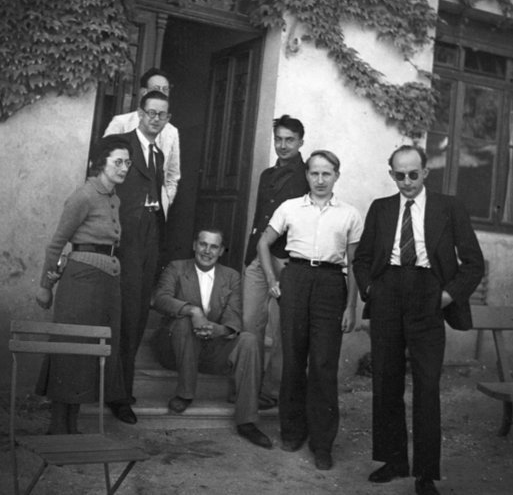
\includegraphics[width=\linewidth]{Bourbaki_congress1938.png}
Bourbaki in Dieulefit\end{minipage}
        }[7]
Let $p$ be a prime of good reduction for $X$ assume we have a \(\QQ_p\)-linear assignment \(\int_b^x :\Omega_{X}^1\otimes \QQ_p \to \QQ_p\) for which:
\[\diff \circ \int_b^x = \mathrm{id},\quad\text{``FTC''}\]%
\[\int_b^x\circ\diff = \mathrm{id}\]%
let $J = \operatorname{Jac}(X)$
% https://q.uiver.app/?q=WzAsNSxbMCwwLCJYKFxcbWF0aGJmIFEpIl0sWzEsMCwiWChcXG1hdGhiZiBRX3ApIl0sWzAsMSwiSihcXG1hdGhiZiBRKSJdLFsxLDEsIkooXFxtYXRoYmYgUV9wKSJdLFsyLDEsIkxpZSBKIChRKSJdLFswLDEsIiIsMCx7InN0eWxlIjp7InRhaWwiOnsibmFtZSI6Imhvb2siLCJzaWRlIjoidG9wIn19fV0sWzAsMiwiIiwyLHsic3R5bGUiOnsidGFpbCI6eyJuYW1lIjoiaG9vayIsInNpZGUiOiJ0b3AifX19XSxbMSwzLCIiLDAseyJzdHlsZSI6eyJ0YWlsIjp7Im5hbWUiOiJob29rIiwic2lkZSI6InRvcCJ9fX1dLFsyLDMsIiIsMix7InN0eWxlIjp7InRhaWwiOnsibmFtZSI6Imhvb2siLCJzaWRlIjoidG9wIn19fV0sWzEsNF0sWzMsNF1d
\[\begin{tikzcd}
	{X(\mathbf Q)} & {X(\mathbf Q_p)} \\
    {J(\mathbf Q)} & {J(\mathbf Q_p)} & {\operatorname{Lie} J (\mathbf Q_p)}
	\arrow[hook, from=1-1, to=1-2]
	\arrow[hook, from=1-1, to=2-1]
	\arrow[hook, from=1-2, to=2-2]
	\arrow[hook, from=2-1, to=2-2]
	\arrow[from=1-2, to=2-3]
	\arrow[from=2-2, to=2-3]
\end{tikzcd}\]
We have
\[\overline {J(\mathbf Q)} \cap X(\mathbf Q_p) \supseteq X(\mathbf Q)\]
now if \[r = \operatorname{rank}(J(\mathbf Q)) < g\] then this intersection is finite!
If we can compute these logarithm functions we can potentially find the intersection explicitly.

\section{Number field Chabauty}
If we work over a fixed number field $K$ one can make sense of all of the above, and sometimes one can do better following ideas of Siksek and Wetherell.

If $X/K$ is a curve over a number field $K$ of degree $d$ then \(\Res_{K/\QQ} (X)\)
is a $d$-dimensional projective variety such that
\[V = \Res_{K/\QQ} (X)(\QQ) \leftrightarrow X(K)\]
and
\[A = \Res_{K/\QQ} (\Jac(X))\]
is a $gd$-dimensional abelian variety.
Then the analogous Chabauty diagram is
\[\begin{tikzcd}
	{V(\mathbf Q)} & {V(\mathbf Q_p)} \\
    {A(\mathbf Q)} & {A(\mathbf Q_p)} & {\operatorname{Lie} A (\mathbf Q_p)}
	\arrow[hook, from=1-1, to=1-2]
	\arrow[hook, from=1-1, to=2-1]
	\arrow[hook, from=1-2, to=2-2]
	\arrow[hook, from=2-1, to=2-2]
	\arrow[from=1-2, to=2-3]
	\arrow[from=2-2, to=2-3]
\end{tikzcd}\]
where now
\[\dim \overline{A(\QQ)} = \rank(J(K)),\,
\dim V(\QQ) = d\]

If \(d + r \le gd \) then we might \emph{hope} that the intersection of these two subspaces is finite, and we can therefore cut out $X(K)$ whenever
\(r \le (g - 1)[K : \QQ]\).

%
%\InsertBoxR{0}{
%    \begin{tikzpicture}[scale=3,
%  line cap=but,
%  l/ine join=round,
%  x=.5em,
%  ultra thick,
%  y=1*(height("Z")-\pgflinewidth)*(1-sin(10)),
%  rotate=-10,
%  rounded corners=1.5pt,
%]\draw (1, 0) -- (0, 0) -- (1, 1) -- (0, 1);\end{tikzpicture}}[4]
\begin{warning}
    The intersection is not always finite! This was noted by Siksek, but even Siksek's guess for a sufficient condition also turned out to be false, as shown by Dogra, with the example of a genus 3 hyperelliptic curve over $\QQ(\sqrt{33})$.
\end{warning}

Nevertheless in practice this approach is quite useful, Siksek gives an explicitly checkable condition that can be used to verify that rational points are alone in their residue disk.

\begin{theorem*}[Siksek]
    For every $X/K$ and $Q \in X(K)$ there is an effectively computable matrix $M_p(Q)$ defined using the integrals of holomorphic 1-forms against a basis of a free subgroup of finite index in $J(K)$, and the local behaviour of the basis of 1-forms such that, if the reduction of $M_p(Q)$ has rank $d$ then $Q$ is the only $K$-rational point of the curve in a $p$-adic unit ball around $Q$.
\end{theorem*}

\begin{example*}[B.--Dahmen]
    Consider \(X\colon  x^{13} + y^{13} = z^5\), one of the generalized Fermat curves, then there exists a covering map
    \[X \to C \colon y^2 = 4 x^5 + 1677 \alpha^2 - 2769 \alpha + 637/K\]
    where
    \[K = \QQ(\alpha ) = \QQ[x]/(x^{3} - x^{2} - 4 x - 1)\]
    is the unique cubic subfield of $\QQ(\zeta _{13})$.
    This curve has rank 2 over $K$ and genus 2, so regular Chabauty does not apply.
    Nevertheless Siksek's techniques using the prime $47$ suffice to show that there are only five $K$-rational points on $C$.
\end{example*}

\emph{Problem:} There are too many functions satisfying all the conditions above, so computing one of them on the nose is hard

\emph{Coleman's idea:} impose that the integral pullback along rigid analytic maps, including for a chosen lift of Frobenius
\[\int_b^x \phi^*\omega = \phi^*\int_b^x \omega\,\quad\text{``Frobenius equivariance''}\]%

We \emph{can} compute the abelian integrals needed for Chabauty by multiplying points on our curve till they lie in the same residue disk on the Jacobian.
%Either we multiply by a very large number (gcd of all possible orders of abvars)

But we would also like for some applications to compute iterated integrals, using Coleman integrals as coefficient functions for 1-forms and iterating again.

To do this, we cannot allow arbitrary rigid functions on our space, but must remove a finite union of disks and consider overconvergent functions:

   \InsertBoxR{0}{\begin{minipage}{0.31\linewidth}
           \centering
           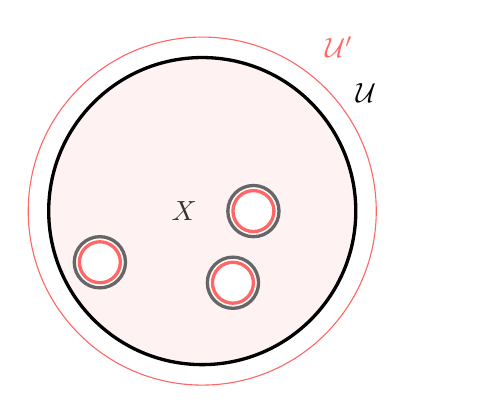
\begin{tikzpicture}[scale=1.3]
               \filldraw[color=black, fill=red!5, very thick](0,0) circle (1.5);
               \node[text width=1.3cm,color=red!60] at (1.7,1.6) {$\mathcal U'$};
               \draw[color=red!60](0,0) circle (1.7);
               \node[text width=1.3cm,color=black] at (2.0,1.15) {$\mathcal U$};
               \filldraw[color=black!60, fill=white, very thick](0.5,0) circle (0.25);
               \filldraw[color=red!60, fill=white, very thick](0.5,0) circle (0.20);
               \filldraw[color=black!60, fill=white, very thick](0.3,-0.7) circle (0.25);
               \filldraw[color=red!60, fill=white, very thick](0.3,-0.7) circle (0.20);
               \filldraw[color=black!60, fill=white, very thick](-1,-0.5) circle (0.25);
               \filldraw[color=red!60, fill=white, very thick](-1,-0.5) circle (0.20);
               \node[text width=1.3cm,color=black!80] at (0.2,0.0) {$X$};
           \end{tikzpicture}
       \end{minipage}%
   }[7]

For example in this way $p$-adic polylogarithms may be defined

$$
\polylog_n (z) = \int \polylog_{n-1}(z) \frac{\diff z}{z},\, \polylog_1(z) = -\log(1-z)
$$

Algorithms to compute these are due to Besser and de Jeu.



\emph{Applications of this theory:}

Coleman integration can be used to define $p$-adic regulators, $p$-adic heights, $p$-adic periods.


\InsertBoxR{-1}{\begin{minipage}{0.30\linewidth}
            \centering
        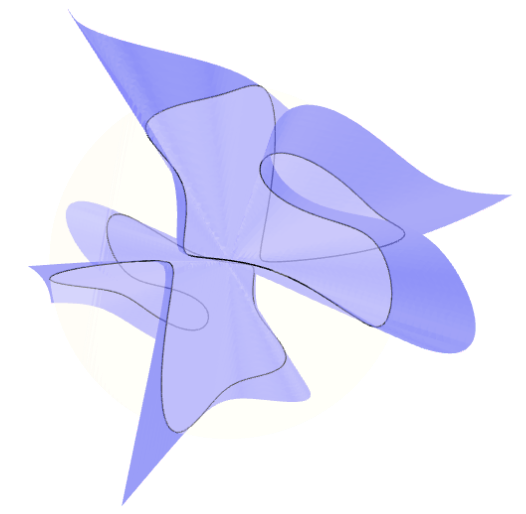
\includegraphics[width=\linewidth]{CartanSurface.png}
Cursed curve by S. Hashimoto\end{minipage}
        }[7]

Of these, $p$-adic heights can be expressed in terms of double integrals and have played a big role in the effort of several authors that enables the non-abelian Chabauty of Kim to be made effective and computable, some highlights:

\emph{Theorem} (Balakrishnan–Dogra–M\"uller–Tuitman–Vonk).
    The (non-)split Cartan modular curve of level 13 is a genus 3 curve which can be given as
    \[\begin{aligned}
        X_s (13) \colon  &y^{4}+5 x^{4}-6 x^{2} y^{2}+6 x^{3} z+26 x^{2} y z+10 x y^{2} z- \\
&10 y^{3} z-32 x^{2} z^{2}-40 x y z^{2}+24 y^{2} z^{2}+32 x z^{3}-16 y z^{3}=0
    \end{aligned}\]
its Jacobian has rank 3, and Picard rank 3.
Then quadratic Chabauty shows that there are exactly 7 rational points on this curve.

\begin{theorem*}[Balakrishnan--B.--Bianchi--Lawrence--Müller--Triantafillou--Vonk]
The number of rational points on the Atkin--Lehner quotient modular curves $X_0(N)^+ := X_0(N)/w_N$, all of genus 2, rank 2 and Picard rank 2 for $N\in \{67, 73, 103\}$ are as follows:
\[ \#X_0(67)^+(\QQ) = 10,\quad \#X_0(73)^+(\QQ) = 10,\quad \#X_0(103)^+(\QQ) = 8.\]
\end{theorem*}

This involves non-abelian Chabauty and Mordell--Weil sieving at $31$ and $137$ in the $N=67$ case.

\begin{theorem*}[Balakrishnan–Dogra–M\"uller–Tuitman–Vonk]
The non-split Cartan modular curve of level 17 is a genus 6 curve, its Jacobian has rank 6.
Quadratic Chabauty shows that there are exactly 7 rational points on this curve.
\end{theorem*}

Many authors by now use quadratic Chabauty computations for interesting questions in rational points,
Adžaga, Arul, Beneish, Chen, Chidambaram, Keller, and Wen
Arul and Müller, Chidambaram, Keller, and Padurariu, and more ...
%TODO more

\emph{Over number fields?} work of Balakrishnan-Besser-Bianchi-Muller caries out explicit quadratic Chabauty over number fields

\emph{Goal:} extend explicit computational tools to general curves over general $p$-adic fields,
to enable experiments and explicit proofs.


\emph{Anatomy of a $p$-adic integral computation:} after Balakrishnan-Bradshaw-Kedlaya

\begin{enumerate}[itemsep=-5mm]
    \item Pick a lift of the Frobenius map
    \item Compute Frobenius action on $H^1$
    \item Evaluate primitives for at least one point in each disk
    \item Compute integrals between nearby points
    \item Solve a linear system
\end{enumerate}
\begin{table}[h!]
    \begin{tabular}{p{60mm}p{60mm}ll}
        Authors                       & Capabilities                                                 & System      \\ \hline
        Balakrishnan-Bradshaw-Kedlaya & Odd hyperelliptic curves / $\QQ_p$                                & Sage       \\
        Balakrishnan-Tuitman (BT)     & General curves with a map to $\mathbf{P}^1$ / ramified & Magma  \\
        B.                            & Superelliptic curves / $\QQ_{p^n}$ (some restriction on $p$)                         & Julia/Nemo  \\
        B.-Kaya-Keller(+CMM) (after BT)     & General curves with a map to $\mathbf{P}^1$ / mixed          & Magma   
    \end{tabular}
\end{table}

In the algorithm of Balakrishnan-Tuitman and BKK we work with almost any plane model of a curve, over a number field $K$, of the form
$$X \colon Q(x,y) = 0.$$
(For now we assume $p$ inert in $K$ and take the completion $K_p \simeq \QQ_{p^n}$)

We consider this together with a map $X \xmapsto{x} \mathbf P^1$.

We work in the ring $R^\dagger/K_p$ of overconvergent $p$-adic functions away from the ramification locus.

Then using prior work of Tuitman we can find a Frobenius lift
$$\phi \colon R^\dagger \to R^\dagger$$
$$x\mapsto x^p$$
$$c \mapsto \sigma (c)\text{ for }c \in \QQ_{p^n},$$
a vector of primitives and the matrix capturing the Frobenius action on cohomology
$$
(\phi ^* \omega _i)_i  = M(\omega _i)_i + \underbrace{(\diff f_i)_i}_{=0} \in H^1_{rig}(X\otimes K_p)\text{.}
$$
these can be computed for a basis $(\omega_i)_i$ of 1-forms $p$-adically integral on the complement of the ramification locus.

Roughly, these algorithms (based on Kedlaya's) approximate the Frobenius lift applied to differentials, then try to iteratively reduce the degree of the resulting series by subtracting appropriately chosen exact differentials.
Generally need to consider many terms!

\emph{Over extension fields:}
In order to integrate over $\QQ_{p^n}$ we start with the known data above.
Assuming we want to integrate between two points of $X(\QQ_{p^n})$.

We define the action of \(\phi \) on \(X(\overline {\QQ}_{p^n})\) via%
\begin{equation*}
\phi (x_0, y_0) = (\sigma \inv (\phi (x) (x_0, y_0)), \sigma \inv (\phi (y)(x_0,y_0)))\text{.}\label{x:men:eqn-pt-act}
\end{equation*}
%
\par
On functions \(f\colon X(\overline{\QQ}_{p^n}) \to \overline{\QQ}_{p^n}\) the action of \(\phi \) is then%
\begin{equation*}
\phi (f)(P) = \sigma f(\phi (P))\text{.}\label{x:men:eqn-fun-act}
\end{equation*}

The action the \(n\)th power of Frobenius on the basis differentials is given by%
\begin{equation*}
\phi ^{*n} (\omega_i)_i  = \sum_{t = n-1,\ldots, 0} \left(\prod_{s=n-1, \ldots, t+1} \sigma^s(M)\right)\phi ^{*t}(\diff f_i)_i + \prod_{s = n-1, \ldots, 0}\sigma ^s(M) (\omega _i)_i\text{.}\label{x:men:eqn-nth-power-frob-act}
\end{equation*}
so that
\begin{gather*}
\left(1 - \prod_{s = n-1, \ldots, 0}\sigma ^s(M)\right) \left(\int_{P}^{Q}\omega _i \right)_i = \label{g:mrow:idm445039011104}\\
\left(\int_P^{\phi ^{n}P} \omega _i\right)_i+ \left(\int_{\phi ^{n} Q}^Q \omega _i\right)_i         + \sum_{t = n-1,\ldots, 0} \left(\prod_{s=n-1, \ldots, t+1} \sigma^s(M)\right)\sigma^t\left(f_i(\phi ^t Q) - f_i(\phi ^t P)\right)_i\text{.}\label{x:mrow:eqn-final-linear}
\end{gather*}
\par

   \InsertBoxR{0}{\begin{minipage}{0.31\linewidth}
           \centering
           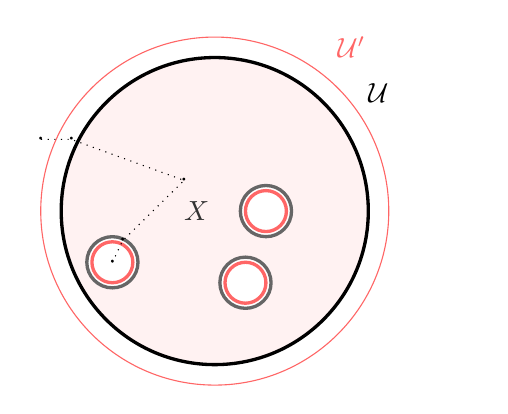
\begin{tikzpicture}[scale=1.3]
               \filldraw[color=black, fill=red!5, very thick](0,0) circle (1.5);
               \node[text width=1.3cm,color=red!60] at (1.7,1.6) {$\mathcal U'$};
               \draw[color=red!60](0,0) circle (1.7);
               \node[text width=1.3cm,color=black] at (2.0,1.15) {$\mathcal U$};
               \filldraw[color=black!60, fill=white, very thick](0.5,0) circle (0.25);
               \filldraw[color=red!60, fill=white, very thick](0.5,0) circle (0.20);
               \filldraw[color=black!60, fill=white, very thick](0.3,-0.7) circle (0.25);
               \filldraw[color=red!60, fill=white, very thick](0.3,-0.7) circle (0.20);
               \filldraw[color=black!60, fill=white, very thick](-1,-0.5) circle (0.25);
               \filldraw[color=red!60, fill=white, very thick](-1,-0.5) circle (0.20);
               \node[text width=1.3cm,color=black!80] at (0.2,0.0) {$X$};
               \draw[dotted] (-1,-0.5) node  {$\cdot$} -- (-0.9,-0.29) node  {$\cdot$} -- (-0.3,0.3) node  {$\cdot$}-- (-1.4,0.7) node  {$\cdot$}-- (-1.7,0.7)node  {$\cdot$};
           \end{tikzpicture}
       \end{minipage}%
   }[7]

As we can compute the RHS and the matrix $M$ we can compute the integrals of basis differentials.

The primitives $f_i$ must be evaluated at at least one point in each disk, and at Frobenius images of these points.

This forces us to pass to a totally ramified extension on top of the unramified one we started with.
We simply choose $\phi$ to be an element of the Galois group of this extension that extends the usual Frobenius on the unramified extension.

In the algorithm for superelliptic curves the superelliptic automorphism is used to conclude that integrals between the bad points all vanish and avoid passing to additional ramified extensions.


\emph{Conclusion:} The algorithm of Balakrishnan-Tuitman can be extended to completely general $p$-adic fields, but remains quite time consuming.

We have a working implementation, and will soon release a preprint with proofs of correctness and complexity analysis.
The Coleman integral is Galois equivariant, which is convenient to check that the implementation is correct, but doesn't seem to help yet when computing.
%\emph{Remark:} This coincides with other forms of $p$-adic integration, such as Colmez's.

%Do you have interesting examples for us (curves over $\QQ(\sqrt{-163}) $)!?


\emph{Time for something completely different:}
A Wieferich prime is one for which
$$2^{p-1} \equiv 1 \pmod{p^2},$$
only 2 are known, unlikely $p$-adic closeness.

Katz (2015) reinterprets this as the fact that $2^{\#\mathbf G_m(\mathbf F_p)}$ is closer to the identity $p$-adically than it is forced to be.

If we assume that this happens no more often that it would randomly we get a heuristic for the distribution of Wieferich primes.

Generalizing we consider an abelian variety $A$ and select an integral model of the Lie algebra of the Neron model and a point $P$ of infinite order, consider
\begin{equation*}
    W_P \colon \{p : p\text{ prime},\, p\text{ good}\} \to \LLie(\mathcal A/\ZZ) \otimes_\ZZ (\RR/\ZZ) \cong (\RR/\ZZ)^d\\
\end{equation*}
\begin{equation*}
    p \mapsto\left(\left(\int^{\#\mathcal A_{\mathbf F_p}(\FF_p)P}_0 \omega _i\right)/p \mod p\right)_i
\end{equation*}
we call this quantity $W_P(p)$ the \emph{Wieferich quotient}, the ``first digit'' of the integral.

Katz conjectures that as long as $P$ generates a Zariski dense subgroup, if we take larger $p$ the Wieferich quotients equidistribute.

The genus 2 curve
\begin{equation*}
X\colon  y^2 = 4x^5 - 8x^4 + 8x^3 - 4x^2 + 1
\end{equation*}
\href{https://www.lmfdb.org/Genus2Curve/Q/997/b/997/1}{997.b.997.1}, has a rational point \(x = (0,1)\) such that the class \(P = \lb x - \infty \rb \in \Jac(X)(\QQ)\) is of infinite order.
A histogram of Wieferich quotients of the Coleman integrals of invariant 1-forms is as follows:

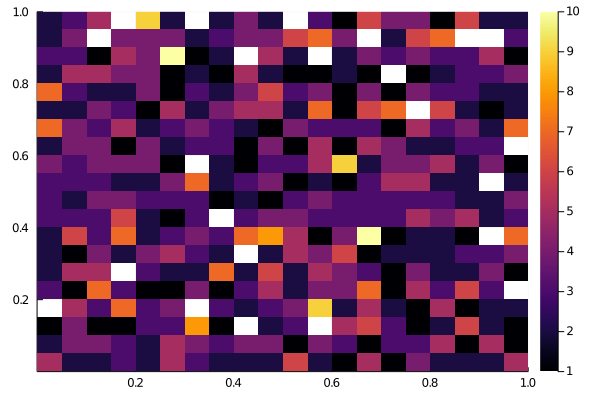
\includegraphics[width=0.9\linewidth]{997.png}

for the Wieferich quotients \(W_P(p)\) for all primes \(15 \lt  p \lt  10000\), and \(p \ne 997\).%

However for the genus 2 curve%
\begin{equation*}
X\colon  y^2 = 4x^5 - 8x^4 + 8x^3 - 4x^2 + 1
\end{equation*}
\href{https://www.lmfdb.org/Genus2Curve/Q/2080/a/4160/2}{2080.a.4160.2}, with \(P = \lb (0,1) - \infty \rb \in \Jac(X)(\QQ)\) of infinite order, the Wieferich quotients \(W_P(p)\) for all primes \(15 \lt  p \lt  10000\).

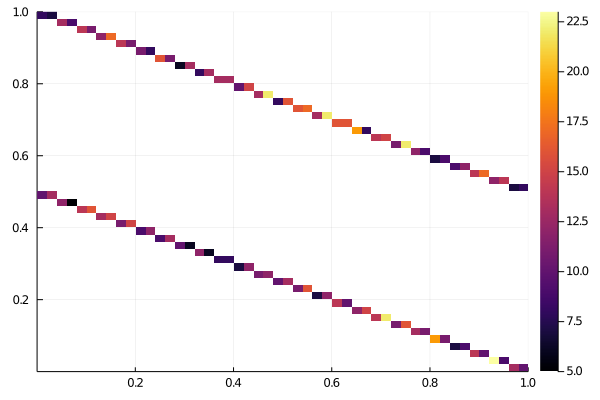
\includegraphics[width=0.9\linewidth]{2080.png}

This curve has Jacobian over \(\QQ\) isogenous the product of elliptic curves 32.a and 65.a. As 32.a is rank 0, the point \(P\) will not generate a Zariski dense subgroup of the Jacobian in this case.%

We see that the annihilating differential is (mod $p$)
\begin{equation*}
\frac{\diff x}{y} +  2x\frac{\diff x}{y}
\end{equation*}
for all these $p$, so almost certainly a global annihilating differential.

Doing these computations type of we gain some evidence for Katz's conjecture, even in cases where other things might interfere, e.g. CM.

\end{document}
